
\documentclass[letterpaper, 12pt]{article}

\usepackage{graphicx}
\usepackage{longtable}
\usepackage{rotating}
\usepackage{dcolumn}
\usepackage{listings}

% Code listing commands
\lstset{language=R,
basicstyle=\scriptsize\ttfamily,
commentstyle=\ttfamily,
numbers=left,
numberstyle=\footnotesize,
stepnumber=1,
numbersep=5pt,
showspaces=false,
showstringspaces=false,
showtabs=false,
frame=single,
tabsize=2,
captionpos=b,
breaklines=true,
breakatwhitespace=false,
title=\lstname,
escapeinside={},
keywordstyle={},
morekeywords={}
}

\begin{document}
\title{ARE213 Problem Set \#1A}
\author{Peter Alstone \& Frank Proulx}
\maketitle

\section{Problem \#1}
\subsection{Part A}

Data records are excluded from the dataset based whether the following variables take the noted values as found in the data manual (see code for implementation).

\subsection{Part B}
We dropped all rows where any data were missing in that row.  One way that the data cleaning process could be improved would be to only remove records based on the variables of interest (as are determined in subsequent analysis) since missing values in fields that are not eventually used in the analysis do not pose a problem..  This would result in a more iterative approach, however, and increase workload on the researcher.

We used some exploratory analysis to understand if the records that were dropped due to missing data \textit{somewhere} in the record were representative.  First we compared a few simple summary statistics between the "full record" and "partial record" data on variables of interest for this analysis.  These are summarized in Table \ref{tab:compareMissingData}.  Better APGAR scores and lower incidence of smoking may be correlated with having full datasets, which indicates the people who have missing data may bias the sample.  We also used agnostic linear regression to understand the relationship between the presence of full records and three key variables: one-minute apgar (omaps), five-minute apgar (fmaps), and number of cigarettes smoked each day (cigar).  The results summarized in Table \ref{tab:lmMissingData} indicate there is statistical significance in each of the factors (i.e. all three are useful predictors for whether a person has a full data record) but also that the influence of the factors is small.  Figure \ref{fig:cigarFullData} shows the distribution in the number of cigarettes smoked by those with and without full records.  The distribution of values is basically the same (clusters around multiples of five up to 20, or, a "pack a day") between the two datasets.  

Overall, in spite of the bias from removing heavier smokers with lower apgar scores from the data, the overall number removed is relatively small and the size of the bias (indicated by the coefficients in the linear model) is relatively small.  

% Table created by stargazer v.4.0 by Marek Hlavac, Harvard University. E-mail: hlavac at fas.harvard.edu
% Date and time: Thu, Sep 19, 2013 - 16:27:57
\begin{table}[!htbp] \centering 
  \caption{Comparison of data with full records to those with missing data across key variables} 
  \label{tab:compareMissingData} 
  \footnotesize
\begin{tabular}{@{\extracolsep{5pt}} ccccccc} 
\\[-1.8ex]\hline 
\hline \\[-1.8ex] 
full.record & mean.omaps & sd.omaps & mean.fmaps & sd.fmaps & mean.cigar & sd.cigar \\ 
\hline \\[-1.8ex] 
FALSE & $7.905$ & $1.572$ & $8.880$ & $1.030$ & $3.945$ & $7.422$ \\ 
TRUE & $8.117$ & $1.260$ & $9.009$ & $0.707$ & $1.907$ & $5.297$ \\ 
\hline \\[-1.8ex] 
\end{tabular} 
\end{table} 


% Table created by stargazer v.4.0 by Marek Hlavac, Harvard University. E-mail: hlavac at fas.harvard.edu
% Date and time: Thu, Sep 19, 2013 - 16:32:14
\begin{table}[!htbp] \centering 
  \caption{Linear model results for predicting whether full records are present based on selected variable of interest in the dataset} 
  \label{tab:lmMissingData} 
\begin{tabular}{@{\extracolsep{5pt}}lc} 
\\[-1.8ex]\hline 
\hline \\[-1.8ex] 
 & \multicolumn{1}{c}{\textit{Dependent variable:}} \\ 
\cline{2-2} 
\\[-1.8ex] & full.record \\ 
\hline \\[-1.8ex] 
 omaps & 0.002$^{***}$ \\ 
  & (0.001) \\ 
  & \\ 
 fmaps & 0.007$^{***}$ \\ 
  & (0.001) \\ 
  & \\ 
 cigar & $-$0.003$^{***}$ \\ 
  & (0.0001) \\ 
  & \\ 
 Constant & 0.882$^{***}$ \\ 
  & (0.007) \\ 
  & \\ 
\hline \\[-1.8ex] 
Observations & 119,384 \\ 
R$^{2}$ & 0.007 \\ 
Adjusted R$^{2}$ & 0.007 \\ 
Residual Std. Error & 0.195 \\ 
F Statistic & 276.305 \\ 
\hline 
\hline \\[-1.8ex] 
\textit{Note:}  & \multicolumn{1}{r}{$^{*}$p$<$0.1; $^{**}$p$<$0.05; $^{***}$p$<$0.01} \\ 
\normalsize 
\end{tabular} 
\end{table}


\begin{figure}[!h] %  figure placement: here, top, bottom, or page
   \centering
   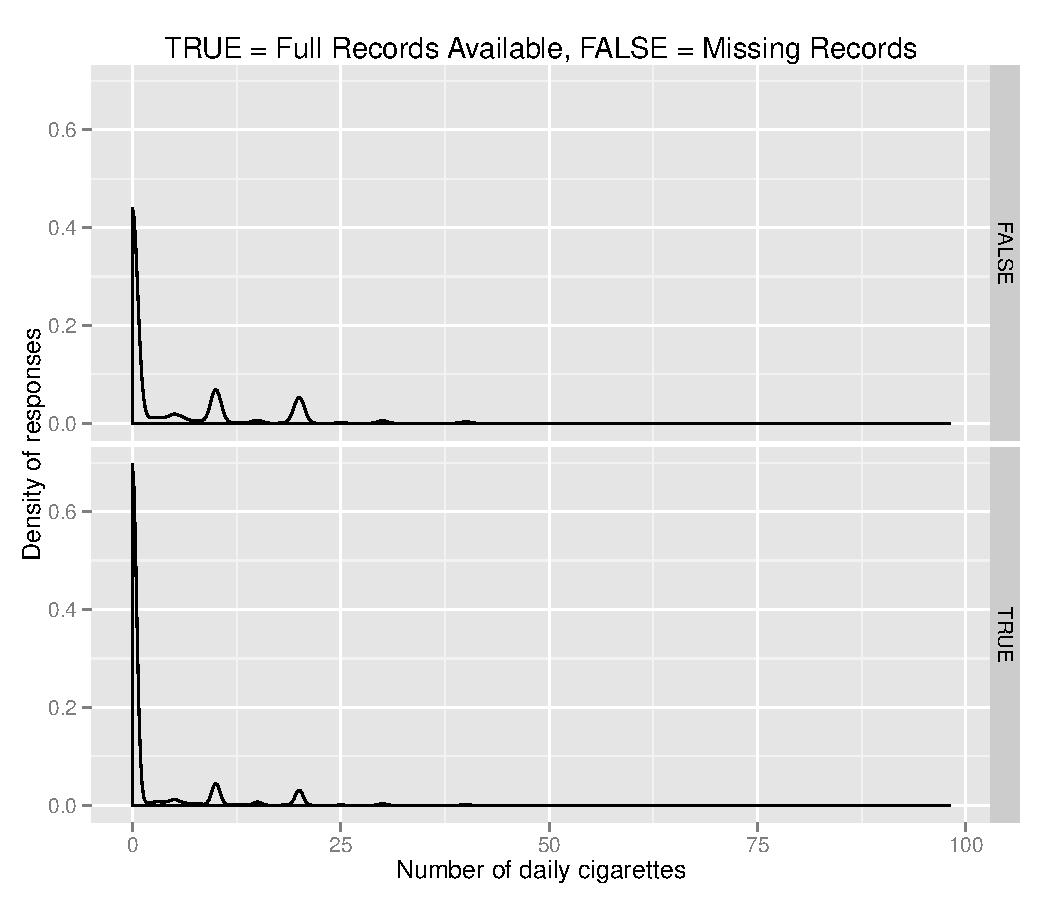
\includegraphics[width=4in]{img/cigar-by-record-type.pdf} 
   \caption{Cigarette use rate by presence of full data record.}
   \label{fig:cigarFullData}
\end{figure}

\subsection{Part C}
Table \ref{tab:summaryClean} is a summary for the remaining data after cleaning.
% Code for the summary table from file summarytable.tex starts here...
% latex.default(summarytable) 
%

% latex.default(title = "variable", file = "clean-summary.tex",      cbind(var.labels, summarytable), caption = "Summary of clean Data",      vbar = TRUE, size = "footnotesize") 
%
\begin{table}[!tbp]
\footnotesize
\caption{Summary of clean data}
\label{tab:summaryClean} 
\begin{center}
\begin{tabular}{|l|l|r|r|r|r|r|}
\hline\hline
\multicolumn{1}{|l|}{variable}&\multicolumn{1}{c|}{var.labels}&\multicolumn{1}{c|}{var}&\multicolumn{1}{c|}{n}&\multicolumn{1}{c|}{mean}&\multicolumn{1}{c|}{sd}&\multicolumn{1}{c|}{se}\tabularnewline
\hline
rectype&record type&$ 1$&$114610$&$   1.26$&$  0.44$&$0.00$\tabularnewline
pldel3&facility of birth recode&$ 2$&$114610$&$   1.02$&$  0.13$&$0.00$\tabularnewline
birattnd&attendant at birth&$ 3$&$114610$&$   1.20$&$  0.56$&$0.00$\tabularnewline
cntocpop&county of occurence&$ 4$&$114610$&$   1.44$&$  1.14$&$0.00$\tabularnewline
stresfip&state of residence&$ 5$&$114610$&$  41.74$&$  2.17$&$0.01$\tabularnewline
dmage&age of mother&$ 6$&$114610$&$  27.76$&$  5.70$&$0.02$\tabularnewline
ormoth&hispanic origin of mother&$ 7$&$114610$&$   0.09$&$  0.52$&$0.00$\tabularnewline
mrace3&race of mother recode&$ 8$&$114610$&$   1.26$&$  0.66$&$0.00$\tabularnewline
dmeduc&detailed educ of mother&$ 9$&$114610$&$  13.21$&$  2.27$&$0.01$\tabularnewline
dmar&marital status of mother&$10$&$114610$&$   1.25$&$  0.43$&$0.00$\tabularnewline
adequacy&adequacy of care recode&$11$&$114610$&$   1.30$&$  0.55$&$0.00$\tabularnewline
nlbnl&number of live births, now living&$12$&$114610$&$   0.97$&$  1.15$&$0.00$\tabularnewline
dlivord&number of live births, now dead&$13$&$114610$&$   1.99$&$  1.17$&$0.00$\tabularnewline
dtotord&detail total birth order&$14$&$114610$&$   2.42$&$  1.52$&$0.00$\tabularnewline
totord9&total birth order recode&$15$&$114610$&$   2.41$&$  1.46$&$0.00$\tabularnewline
monpre&month pregnancy prenatal care began&$16$&$114610$&$   2.50$&$  1.33$&$0.00$\tabularnewline
nprevist&total number of prenatal visits&$17$&$114610$&$  11.15$&$  3.52$&$0.01$\tabularnewline
disllb&interval since last live birth&$18$&$114610$&$ 350.41$&$362.33$&$1.07$\tabularnewline
isllb10&interval since last live birth recode&$19$&$114610$&$   3.32$&$  3.19$&$0.01$\tabularnewline
dfage&age of father&$20$&$114610$&$  30.06$&$  6.41$&$0.02$\tabularnewline
orfath&hispanic origin of father&$21$&$114610$&$   0.09$&$  0.53$&$0.00$\tabularnewline
dfeduc&educ of father detail&$22$&$114610$&$  13.28$&$  2.33$&$0.01$\tabularnewline
birmon&month of birth&$23$&$114610$&$   6.47$&$  3.39$&$0.01$\tabularnewline
weekday&day of week child born&$24$&$114610$&$   4.05$&$  1.88$&$0.01$\tabularnewline
dgestat&gestation -- detail in weeks&$25$&$114610$&$  39.15$&$  2.44$&$0.01$\tabularnewline
csex&sex of child&$26$&$114610$&$   1.49$&$  0.50$&$0.00$\tabularnewline
dbrwt&birthweight in grams&$27$&$114610$&$3373.29$&$585.17$&$1.73$\tabularnewline
dplural&plurality&$28$&$114610$&$   1.03$&$  0.17$&$0.00$\tabularnewline
omaps&one minute agpar score&$29$&$114610$&$   8.12$&$  1.26$&$0.00$\tabularnewline
fmaps&five minute agpar score&$30$&$114610$&$   9.01$&$  0.71$&$0.00$\tabularnewline
clingest&clinical estimate of gestation&$31$&$114610$&$  39.11$&$  2.06$&$0.01$\tabularnewline
delmeth5&method of delivery&$32$&$114610$&$   1.55$&$  1.01$&$0.00$\tabularnewline
anemia&anemia mother&$33$&$114610$&$   1.99$&$  0.10$&$0.00$\tabularnewline
cardiac&cardiac disease mother&$34$&$114610$&$   1.99$&$  0.08$&$0.00$\tabularnewline
lung&acute or chronic lung disease mother&$35$&$114610$&$   1.99$&$  0.08$&$0.00$\tabularnewline
diabetes&diabetes mother&$36$&$114610$&$   1.97$&$  0.16$&$0.00$\tabularnewline
herpes&genital herpes mother&$37$&$114610$&$   1.99$&$  0.08$&$0.00$\tabularnewline
chyper&chronic hypertension&$38$&$114610$&$   1.99$&$  0.09$&$0.00$\tabularnewline
phyper&pregnancy related hypertension&$39$&$114610$&$   1.97$&$  0.17$&$0.00$\tabularnewline
pre4000&previous infant 4000 or more grams&$40$&$114610$&$   1.99$&$  0.12$&$0.00$\tabularnewline
preterm&previous preterm infant&$41$&$114610$&$   1.99$&$  0.12$&$0.00$\tabularnewline
tobacco&tobacco use during pregnancy&$42$&$114610$&$   1.84$&$  0.37$&$0.00$\tabularnewline
cigar&average number of cigarettes per day&$43$&$114610$&$   1.91$&$  5.30$&$0.02$\tabularnewline
cigar6&average number of cigarettes per day recode&$44$&$114610$&$   0.35$&$  0.86$&$0.00$\tabularnewline
alcohol&alcohol use during pregnancy&$45$&$114610$&$   1.99$&$  0.10$&$0.00$\tabularnewline
drink&average number of drinks per week&$46$&$114610$&$   0.03$&$  0.62$&$0.00$\tabularnewline
drink5&average number of drinks recode&$47$&$114610$&$   0.02$&$  0.23$&$0.00$\tabularnewline
wgain&weight gain&$48$&$114610$&$  30.36$&$ 11.88$&$0.04$\tabularnewline
full.record*&full record present&$49$&$114610$&$   1.00$&$  0.00$&$0.00$\tabularnewline
\hline
\end{tabular}
\end{center}
\end{table}

 % need to fix this table so it is more visible...currently runs off the page.  

\section{Problem \#2}

\subsection{Part A}

The table below shows the mean differences between smoking and non-smoking mothers for one-minute APGAR scores (ompas), five-minute (fmaps), and birth weight in grams (dbrwt).  Unconditioned on the other variables, there is no statistically significant difference in APGAR score but a significant difference is present in birth weight\footnote{Welch Two Sample t-test, alternative hypothesis: true difference in means is not equal to 0; p-value less than 2.2e-16, 95 percent confidence interval: -249.5463 to -231.4093}.   

% Table created by stargazer v.4.0 by Marek Hlavac, Harvard University. E-mail: hlavac at fas.harvard.edu
% Date and time: Sat, Sep 21, 2013 - 00:11:19
\begin{table}[!htbp] \centering 
  \caption{Comparison of key birthing infant health indicators for different maternal smoking status} 
  \label{} 
\begin{tabular}{@{\extracolsep{5pt}} cccc} 
\\[-1.8ex]\hline 
\hline \\[-1.8ex] 
tobacco & mean.omaps & mean.fmaps & mean.dbrwt \\ 
\hline \\[-1.8ex] 
smoker & 8.10 & 9.01 & 3171 \\ 
nonsmoker & 8.12 & 9.01 & 3412 \\ 
difference & 0.017 & 0.0001 & 240.5 \\ 
\hline \\[-1.8ex] 
\normalsize 
\end{tabular} 
\end{table} 


\subsection{Part B}

The average treatment effect (ATE) of maternal smoking can only be determined by comparing the unadjusted difference in mean birth weight of infants \textbf{if their mothers were randomly assigned into treatment (a smoking habit during pregnancy) or the assignment / selection to treatment is as good as random}.  This is obviously not possible or even palatable for a variety of practical and ethical reasons to verify with RCT so an alternative approach to identifying the ATE that controls for observables is the next-best option.  If we assume that smoking habits are randomly assigned among pregnant mothers, it can be "safe" to use the unadjusted difference in weight as a predictor of ATE without conditioning on observables as long as there are not any significant differences in the smoking and non-smoking groups that also influence birth weight.  In the next set of steps we explore other factors that may influence birth weight and if they are also related to smoking status.  
  

\paragraph{ATE using unadjusted differences:}
If we were to assume that smoking is in fact randomly assigned, the mean difference in birth weight caused by smoking between infants whose mothers smoke and those who do not is 240 grams (with a 95\% confidence interval of 230 - 250 grams). Infants whose mother smoked have about  7\% lower birth weight than those who did not. \newline{}


\paragraph{Identifying potential confounding factors:}
We used deductive logic and graphical exploration to understand factors that may influence birth weight and should be controlled for if the tobacco users / non-users have distributions that are not identical (or very similar) between them.  Several (but not all) of the factors that we identified as potential candidates are summarized in the Table \ref{tab:xtabsTobacco}.  We omitted many that did not show a relationship between the factor and birth weight for brevity.  The results show that most of the potential factors related to birth weight do not appear likely to be also related to smoking status.  \newline

% latex.default(cstats, title = title, caption = caption, rowlabel = rowlabel,      col.just = col.just, numeric.dollar = FALSE, insert.bottom = legend,      rowname = lab, dcolumn = dcolumn, extracolheads = extracolheads,      extracolsize = Nsize, ...) 
%
\begin{table}[!tbp]
\caption{Descriptive Statistics by tobacco\label{crosstab-tobacco}} 
\begin{center}
\begin{tabular}{lccc}
\hline\hline
\multicolumn{1}{l}{}&\multicolumn{1}{c}{smoker}&\multicolumn{1}{c}{nonsmoker}&\multicolumn{1}{c}{Combined}\tabularnewline
&\multicolumn{1}{c}{{\scriptsize $N=18266$}}&\multicolumn{1}{c}{{\scriptsize $N=96344$}}&\multicolumn{1}{c}{{\scriptsize $N=114610$}}\tabularnewline
\hline
mrace3~:~White&87\%~{\scriptsize~(15876)}&86\%~{\scriptsize~(82748)}&86\%~{\scriptsize~(98624)}\tabularnewline
~~~~Other&~0\%~{\scriptsize~(~~~69)}&~2\%~{\scriptsize~(~2202)}&~2\%~{\scriptsize~(~2271)}\tabularnewline
~~~~Black&13\%~{\scriptsize~(~2321)}&12\%~{\scriptsize~(11394)}&12\%~{\scriptsize~(13715)}\tabularnewline
csex~:~Male&52\%~{\scriptsize~(~9462)}&51\%~{\scriptsize~(49505)}&51\%~{\scriptsize~(58967)}\tabularnewline
~~~~Female&48\%~{\scriptsize~(~8804)}&49\%~{\scriptsize~(46839)}&49\%~{\scriptsize~(55643)}\tabularnewline
dplural~:~Singleton&98\%~{\scriptsize~(~17860)}&97\%~{\scriptsize~(~93694)}&97\%~{\scriptsize~(111554)}\tabularnewline
~~~~Twin&~2\%~{\scriptsize~(~~~400)}&~3\%~{\scriptsize~(~~2503)}&~3\%~{\scriptsize~(~~2903)}\tabularnewline
~~~~Triplet&~0\%~{\scriptsize~(~~~~~6)}&~0\%~{\scriptsize~(~~~135)}&~0\%~{\scriptsize~(~~~141)}\tabularnewline
~~~~Quadruplet&~0\%~{\scriptsize~(~~~~~0)}&~0\%~{\scriptsize~(~~~~12)}&~0\%~{\scriptsize~(~~~~12)}\tabularnewline
clingest&{\scriptsize 38~}{40 }{\scriptsize 40} &{\scriptsize 38~}{40 }{\scriptsize 40} &{\scriptsize 38~}{40 }{\scriptsize 40} \tabularnewline
alcohol~:~Drinker&~~3\%~{\scriptsize~(~~~639)}&~~0\%~{\scriptsize~(~~~472)}&~~1\%~{\scriptsize~(~~1111)}\tabularnewline
~~~~Nondrinker&~97\%~{\scriptsize~(~17627)}&100\%~{\scriptsize~(~95872)}&~99\%~{\scriptsize~(113499)}\tabularnewline
dmage&{\scriptsize 22~}{26 }{\scriptsize 30} &{\scriptsize 24~}{28 }{\scriptsize 32} &{\scriptsize 24~}{28 }{\scriptsize 32} \tabularnewline
\hline
\end{tabular}
\end{center}
\noindent {\scriptsize $a$\ }{$b$\ }{\scriptsize $c$\ } represent the lower quartile $a$, the median $b$, and the upper quartile $c$\ for continuous variables.\\Numbers after percents are frequencies.\end{table}

 %Table with sample cross tabs for smoking status and a variety of factors.



The factors we identify as having an impact on birth weight AND being related to smoking status are:

\begin{itemize}

\item \textbf{Maternal Age} is different between the smoking / non-smoking group and is related to birth weight.  The median pregnant smoker is two years younger than the median non-smoker.  There is also a relationship between age and birth weight (where older mothers up to age 31-32 or so tend to have heavier babies).  The relationship between maternal age and birth weight along with the distributions in age for smokers and non-smokers is shown in Figure \ref{fig:bwAge}

\item \textbf{Marital Status} is also different between the smoking and non-smoking groups: single mothers are more likely to smoke in pregnancy.  In the whole sample the fraction of women who are married is 75\% but in the ``smoker'' subsample it is only 52\%.  There is also a relationship between marital status and birth weight whereby married mothers tend to have slightly heavier babies.  These relationships are shown in Figure \ref{fig:bwMar}.  If one believes that being married leads to less stress for mothers and/or better resources and support it is possible that marital status is a proxy for other determinants of infant weight.  However, as is also shown in the Figure (bottom panel) there are different distributions in maternal age between married and unmarried women, with a relationship that suggests age may be a stronger determining factor since single mothers are typically younger than married mothers.   

\item \textbf{Maternal weight gain (less certain)} is related to infant weight at birth but as we note is not as certain in terms of being related strongly with smoking status.  The median weight gain is quite similar between the two smoking status groups (29 lbs for smokers vs. 30 lbs for non-smokers) but there is a larger difference in the 25th percentile weight (20 vs. 24 lbs.).  The relationship between maternal weight gain and infant weight gain along with the distribution in maternal gain by smoking status is summarized in Figure \ref{fig:bwGain}

\begin{figure}[htbp]
\begin{center}
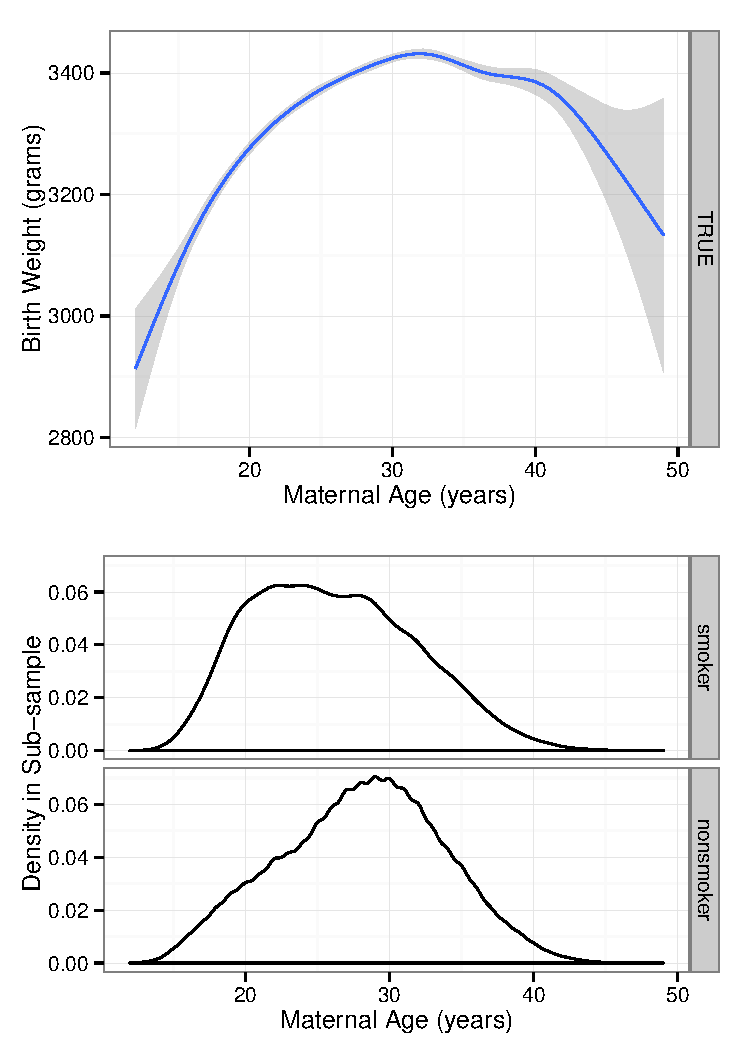
\includegraphics{img/bw-age.pdf}
\caption{(Top) The relationship between Maternal Age and Birth Weight with a GAM fit to the data and 95\% confidence interval estimate in grey.  Actual data are omitted to show the average trend more clearly.  (Bottom panels) A comparison in the distribution of Maternal Age for smokers and non-smokers shows how smokers tend to be younger mothers.}
\label{fig:bwAge}
\end{center}
\end{figure}

\begin{figure}[htbp]
\begin{center}
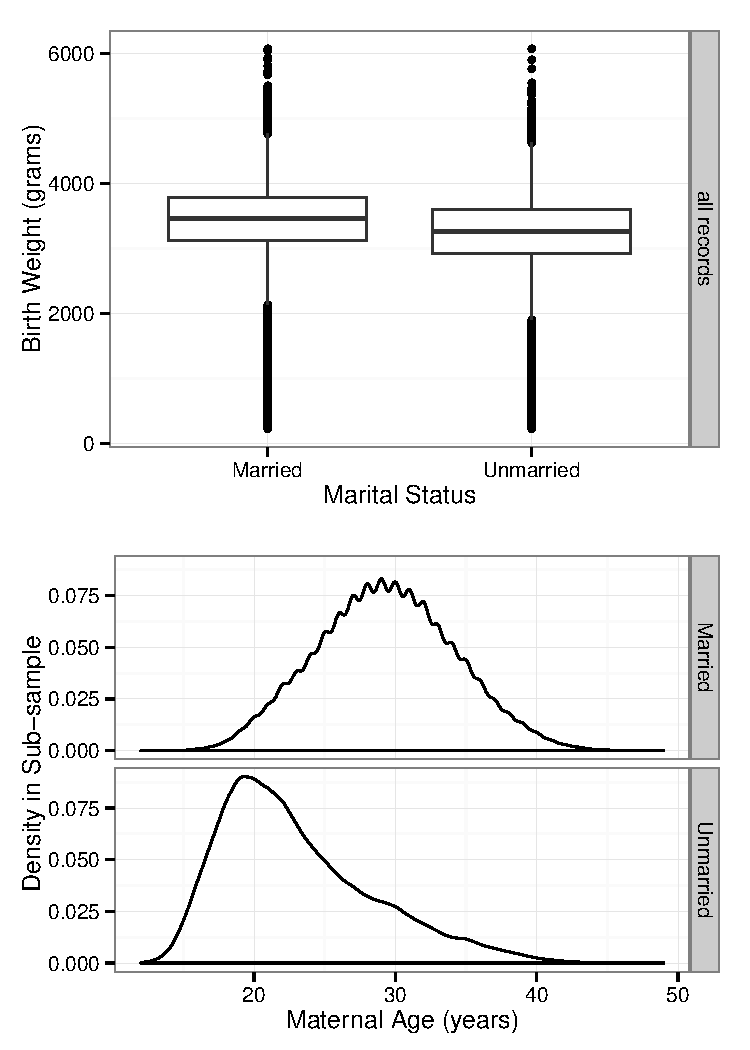
\includegraphics{img/bw-mar.pdf}
\caption{(Top) Boxplots for birth weight by marital status of the mother. (Bottom) Distribution in maternal age between married and unmarried women.}
\label{fig:bwMar}
\end{center}
\end{figure}

\begin{figure}[htbp]
\begin{center}
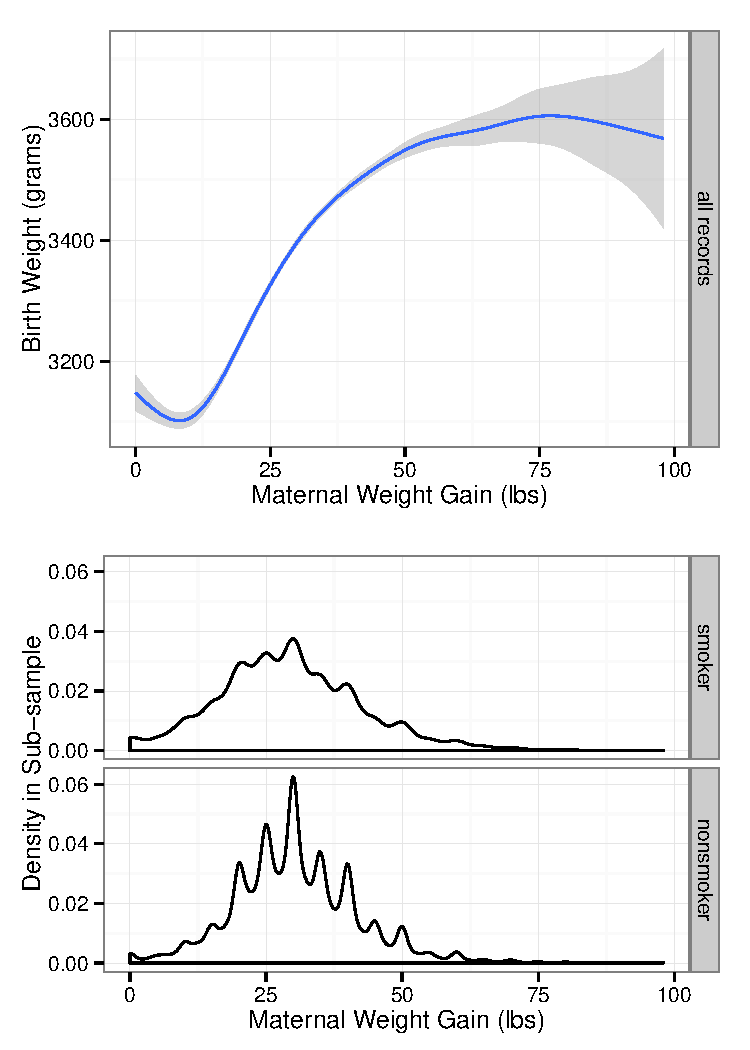
\includegraphics{img/bw-gain.pdf}
\caption{(Top) The relationship between Maternal Weight Gain and Birth Weight with a GAM fit to the data and 95\% confidence interval estimate in grey.  Actual data are omitted to show the average trend more clearly.  (Bottom panels) A comparison in the distribution of Maternal Weight Gain for smokers and non-smokers shows how smokers tend to have (slightly) less weight gain.}
\label{fig:bwGain}
\end{center}
\end{figure}

\end{itemize}

The position that smoking status is randomly assigned may have some rational basis, but we cannot claim complete randomness.  Consider the following line of reasoning:

\begin{itemize}
\item This study was conducted in 1993, decades after the link between smoking and poor infant health was established and widely publicized in both the scientific literature and (more importantly) the popular media.  While there is a link between maternal educational attainment (smokers tend to have less education, slightly), this can largely be explained by the age of the mothers (many of whom are simply too young to have graduated college, etc.).  This education gap could potentially explain a difference in awareness but we posit it is probably a poor proxy.  It is reasonable to expect that the vast majority of mothers in the sample know about the link between smoking during pregnancy and poor infant health outcomes, and that the smoking and non-smoking mothers both have the same maternal drive to protect their unborn infants.

\item Furthermore, even if the popular exposure were different between smokers and non-smokers, it is standard practice during neonatal care to receive messages about the value of not smoking.  Both smokers and non-smokers presumably received roughly the same level of neonatal care (as measured by the month at which care began).  

\item If one accepts that awareness about smoking risk and the level of maternal protection drive is the same in both groups, perhaps the only remaining factors are those that underly addiction: genetic predisposition and environmental factors.  It is possible, but by no means certain, that the genetic factors (at least) are essentially randomly distributed between people.  However, the underlying environmental factors that lead to addiction are not likely randomly distributed and may be correlated with both smoking and other maternal behavior that could lead to lower birth weight.  

\item Based on the above we posit that there is an element of randomness (genetic factors) associated with smoking but that environmental factors (education, upbringing, social pressures) also contribute strongly to both smoking status and other factors that could cause low birth weight (like pregnancies earlier in life).  

\end{itemize}


Because of the factors we identified it is not defensible to grant the assumption that smoking is randomly assigned in the population.  Using unadjusted mean differences is not tenable for obtaining an accurate prediction of ATE. 


\subsection{Part C}

An approach to "correcting" for non-random selection to treatment is identifying predetermined (or exogenous) factors and attempting to control them them.  In this case, where we are analyzing data ex post of the "natural experiment" that was documented, we will identify factors that meet three criteria to use as controls: 1) Predetermined or exogenous data, 2) Exhibit some bias in the treatment and control groups, 3) Agnostic to the treatment status, exhibit covariance with birth weight.  \newline

Some variables are clearly not predetermined and are endogenous to treatment.  In general the predetermined factors are those that can be completely extricated from the treatment, i.e., those that could be changed for a particular individual without changing the treatment category.  Factors that are not predetermined, and therefore cannot be pulled apart from treatment effects, are those that derive at least partly from the smoking status of the mother or underlying factors of smoking status.  The ultimate goal is to identify predetermined factors so they can be controlled in the regression to capture only factors that can be effected by the treatment.  \newline

It is helpful in this case to define a time at which treatment "begins."  Since we might be interested to inform public policy, one could investigate potential benefits of a smoking cessation program for women who are trying to conceive children.  Taking this as a benchmark, the experiment we would run, if it were ethical and practical, would be to randomly assign women to either smoke or not smoke just before they became pregnant.  Based on this, any outcome that is related to the mother or child's biology after conception is not predetermined (e.g., maternal weight gain).  Other factors that could not be predetermined in the experiment are pregnancy-related health concerns like hypertension, the month prenatal care began (since a woman who smokes, and knows it is potentially harmful to the infant, may hesitate to seek medical care), alcohol use during pregnancy (people often smoke and drink socially), gestational age at birth, and other medically related indicators.  \newline

There are, however, a range of predetermined factors that could enter the linear model if they meet our other criteria (which are in place to avoid a "crowded / kitchen sink" model that is difficult to describe and interpret): bias in the selection to treatment groups and an obvious influence on birth weight.  \newline

Based on our analysis and reasoning, there are two key factors that are predetermined, contribute to birth weight, and also are biased by the "smoking" treatment: Maternal Age and Marital Status.  Other factors that are predetermined but do not meet the other two criteria (contributing to weight AND biased by smoking treatment comported to the larger sample) include the sex of the baby, level of prenatal care, age of the father (to the extent that there are genetic causes), gestational time, state of residence, infant plurality, etc.  There are also factors that are not predetermined and seem to be (potentially) closely linked with treatment status, such as alcohol use in utero (which was a small fraction of the whole population), maternal weight gain, pregnancy related hypertension, and incidences of lung disease.  \newline


\subsection{Part D}

Selection on observables strategies for teasing out causality guide us to identify all the observable factors (except for the treatment--smoking in this case) that could lead to the outcome (birth weight) and to "correct" for these using statistical techniques before the test for smoking.  We identified three additional key factors above that we will use in a set of simple linear models to understand how different factors influence birth weight: Maternal Age, Marital Status, and Maternal Weight Gain.  We include maternal weight gain with prejudice on how to interpret it because it too could be linked with smoking status (anecdotal evidence indicates that smoking tends to suppress weight gain and that smoking cessation could lead to temporary weight gain).  Table \ref{bwLMNoTob} and \ref{bwLMWithTob} below summarize the suite of linear models we used to explore the relationships between various potential causal factors and birth weight\newline

The outcome of the models indicates that each of the three additional factors (in addition to tobacco use) is statistically significant in terms of predicting birth weight.  However, because maternal weight gain is not a clearly predetermined factor we choose to ignore models that include it (although it is interesting to examine them).  The "best" model that only includes Maternal Age and Marital Status as conditioning variables along with tobacco use.  \newline

By introducing conditioning variables in a linear regression we downgrade the estimate for average treatment effect from 240 grams to about 200 grams because smokers tended to be younger and unmarried (both significantly decrease birth weight).  



% TABLE Birthweight without tobacco.
% Table created by stargazer v.4.0 by Marek Hlavac, Harvard University. E-mail: hlavac at fas.harvard.edu
% Date and time: Mon, Sep 23, 2013 - 11:24:05
% Requires LaTeX packages: dcolumn 
\begin{sidewaystable}[!htbp] \centering 
  \caption{Birth weight linear models without including Tobacco factors} 
  \label{tab:bwLMNoTab} 
\footnotesize 
\begin{tabular}{@{\extracolsep{5pt}}lD{.}{.}{-3} D{.}{.}{-3} D{.}{.}{-3} } 
\\[-1.8ex]\hline 
\hline \\[-1.8ex] 
\\[-1.8ex] & \multicolumn{3}{c}{Birth Weight} \\ 
\\[-1.8ex] & \multicolumn{1}{c}{(1)} & \multicolumn{1}{c}{(2)} & \multicolumn{1}{c}{(3)}\\ 
\hline \\[-1.8ex] 
 Maternal Age & 9.536^{***} & 2.888^{***} & 4.246^{***} \\ 
  & (0.302) & (0.341) & (0.334) \\ 
  & & & \\ 
 Marital Status (unmarried) &  & -183.626^{***} & -175.893^{***} \\ 
  &  & (4.479) & (4.384) \\ 
  & & & \\ 
 Weight Gain &  &  & 10.042^{***} \\ 
  &  &  & (0.141) \\ 
  & & & \\ 
 Constant & 3,108.613^{***} & 3,339.251^{***} & 2,994.784^{***} \\ 
  & (8.558) & (10.190) & (11.081) \\ 
  & & & \\ 
\textit{N} & \multicolumn{1}{c}{114,610} & \multicolumn{1}{c}{114,610} & \multicolumn{1}{c}{114,610} \\ 
R$^{2}$ & \multicolumn{1}{c}{0.009} & \multicolumn{1}{c}{0.023} & \multicolumn{1}{c}{0.064} \\ 
Adjusted R$^{2}$ & \multicolumn{1}{c}{0.009} & \multicolumn{1}{c}{0.023} & \multicolumn{1}{c}{0.064} \\ 
Residual Std. Error & \multicolumn{1}{c}{582.649 (df = 114608)} & \multicolumn{1}{c}{578.426 (df = 114607)} & \multicolumn{1}{c}{566.024 (df = 114606)} \\ 
F Statistic & \multicolumn{1}{c}{996.918$^{***}$ (df = 1; 114608)} & \multicolumn{1}{c}{1,346.077$^{***}$ (df = 2; 114607)} & \multicolumn{1}{c}{2,629.910$^{***}$ (df = 3; 114606)} \\ 
\hline 
\hline \\[-1.8ex] 
\textit{Notes:} & \multicolumn{3}{r}{$^{***}$Significant at the 1 percent level.} \\ 
 & \multicolumn{3}{r}{$^{**}$Significant at the 5 percent level.} \\ 
 & \multicolumn{3}{r}{$^{*}$Significant at the 10 percent level.} \\ 
\normalsize 
\end{tabular} 
\end{sidewaystable} 



%TABLE Birthweight WITH tobacco
% Table created by stargazer v.4.0 by Marek Hlavac, Harvard University. E-mail: hlavac at fas.harvard.edu
% Date and time: Mon, Sep 23, 2013 - 11:35:16
% Requires LaTeX packages: dcolumn 
\begin{sidewaystable}[!htbp] \centering 
  \caption{Birth weight linear models including Tobacco factors} 
  \label{tab:bwLMWithTob} 
\footnotesize 
\begin{tabular}{@{\extracolsep{5pt}}lD{.}{.}{-3} D{.}{.}{-3} D{.}{.}{-3} } 
\\[-1.8ex]\hline 
\hline \\[-1.8ex] 
\\[-1.8ex] & \multicolumn{3}{c}{Birth Weight} \\ 
\\[-1.8ex] & \multicolumn{1}{c}{(1)} & \multicolumn{1}{c}{(2)} & \multicolumn{1}{c}{(3)}\\ 
\hline \\[-1.8ex] 
 Maternal Age & 4.058^{***} & 2.716^{***} & 7.781^{***} \\ 
  & (0.332) & (0.338) & (0.301) \\ 
  & & & \\ 
 Marital Status (unmarried) & -141.095^{***} & -146.507^{***} &  \\ 
  & (4.444) & (4.538) &  \\ 
  & & & \\ 
 Weight Gain & 9.850^{***} &  &  \\ 
  & (0.140) &  &  \\ 
  & & & \\ 
 Tobacco (nonsmoker) & 183.678^{***} & 195.101^{***} & 225.823^{***} \\ 
  & (4.668) & (4.764) & (4.690) \\ 
  & & & \\ 
 Constant & 2,842.679^{***} & 3,170.698^{***} & 2,967.483^{***} \\ 
  & (11.666) & (10.921) & (8.965) \\ 
  & & & \\ 
\textit{N} & \multicolumn{1}{c}{114,610} & \multicolumn{1}{c}{114,610} & \multicolumn{1}{c}{114,610} \\ 
R$^{2}$ & \multicolumn{1}{c}{0.077} & \multicolumn{1}{c}{0.037} & \multicolumn{1}{c}{0.028} \\ 
Adjusted R$^{2}$ & \multicolumn{1}{c}{0.077} & \multicolumn{1}{c}{0.037} & \multicolumn{1}{c}{0.028} \\ 
Residual Std. Error & \multicolumn{1}{c}{562.240 (df = 114605)} & \multicolumn{1}{c}{574.242 (df = 114606)} & \multicolumn{1}{c}{576.845 (df = 114607)} \\ 
F Statistic & \multicolumn{1}{c}{2,386.185$^{***}$ (df = 4; 114605)} & \multicolumn{1}{c}{1,469.452$^{***}$ (df = 3; 114606)} & \multicolumn{1}{c}{1,667.935$^{***}$ (df = 2; 114607)} \\ 
\hline 
\hline \\[-1.8ex] 
\textit{Notes:} & \multicolumn{3}{r}{$^{***}$Significant at the 1 percent level.} \\ 
 & \multicolumn{3}{r}{$^{**}$Significant at the 5 percent level.} \\ 
 & \multicolumn{3}{r}{$^{*}$Significant at the 10 percent level.} \\ 
\normalsize 
\end{tabular} 
\end{sidewaystable}

\pagebreak
\section{[R] Code}

We used R to complete this assignment.  The code is below:

\lstinputlisting{ps1a1.R}

\lstinputlisting{../util/are213-func.R}


\end{document}
